\documentclass[12pt]{article}
\usepackage[top=1in, bottom=1in, left=1.5in, right=1in]{geometry}
\usepackage{graphicx}
\usepackage{listings}
\usepackage{fullpage}
\usepackage{color}
\usepackage{graphicx}
\usepackage{hyperref}
\graphicspath{ ./ }
\renewcommand{\baselinestretch}{1.5} 

\definecolor{codegreen}{rgb}{0,0.6,0}
\definecolor{codegray}{rgb}{0.5,0.5,0.5}
\definecolor{codepurple}{rgb}{0.58,0,0.82}
\definecolor{backcolour}{rgb}{0.95,0.95,0.92}

\lstset{
    backgroundcolor=\color{backcolour},   
    commentstyle=\color{codegreen},
    keywordstyle=\color{magenta},
    numberstyle=\tiny\color{codegray},
    stringstyle=\color{codepurple},
    basicstyle=\tiny,
    breakatwhitespace=false,         
    breaklines=true,                 
    captionpos=b,                    
    keepspaces=true,                 
    numbers=left,                    
    columns=fixed,
    basewidth=.5em,
    numbersep=5pt,                  
    showspaces=false,                
    showstringspaces=false,
    showtabs=false,                  
    tabsize=2
}

\hypersetup{
    colorlinks,
    citecolor=black,
    filecolor=black,
    linkcolor=black,
    urlcolor=black
}

\begin{document}

\begin{titlepage}

\begin{center}

\renewcommand{\baselinestretch}{1.5}
\Large \textbf { A BASIC, FOUR LOGIC CLUSTER, DISJOINT SWITCH CONNECTED FPGA ARCHITECTURE }\\[0.8in]


\normalsize
\textbf{ A SENIOR PROJECT REPORT}\\[0.1in]
 \small
       \textit{\textbf{Submitted in partial fulfillment of
        the requirements for the award of the degree of}}\\[0.3in]
        
\normalsize
       \textbf{ BACHELOR OF SCIENCE \\IN\\ COMPUTER ENGINEERING}\\[0.5in]

% Submitted by
 by \\
\textbf{ JOSEPH PRACHAR }




\vspace{.3in}
Under the guidance of\\
{\textbf{ Dr. Tina Smilkstein }}\\[0.1in]

\vfill

% Bottom of the page

\includegraphics[height=1.8in]{logo}\\[0.1in]
{Department of Computer Engineering}\\
\normalsize
\textsc{ California Polytechnic State University, San Luis Obispo }\\
March 2018\\
\textcolor{red}{\textbf{VERSION 0.1}}


\end{center}

\end{titlepage}

\begin{abstract}
This paper seeks to describe the process of developing a new FPGA architecture from 
nothing, both in terms of knowledge about FPGAs and in initial design material. Specifically,
 this project set out to design an FPGA architecture which could implement a simple 
state machine type design with less than 10 inputs, less than 10 outputs and less 
than 10 states. This project was completed making use of the cadence suite of software 
tools (mainly Gennus, Innovus, and Virtuoso) and Global Foundries CMRF8SF 130nm process.
 This endeavor proved to be too extensive for a seven week quarter and so was unsuccessful 
in meeting the original design goals. However, this project did accomplish creating 
a revised FPGA architecture capable of implementing a state machine with 11 inputs,
 5 outputs, and 32 possible states.
\end{abstract}
\newpage

\tableofcontents
\newpage
\listoffigures
\newpage

\section{Introduction}

\subsection{Overview}

FPGA’s are some of the most complicated digital circuits on the market today. They 
can help companies build a custom digital circuit with years less development time 
compared to a comparable ASIC design process. This project aims to be an initial 
exploratory exercise into the implementation details of the FPGA through the creation 
of a basic FPGA architecture. This new architecture will be extremely basic in nature 
due to the vastly intricate circuit that needs to be created and the complex software 
required to route designs within it.

This project will focus on pulling together the many basic overviews provided by 
the research sources listed in Appendix 1. The main technical overview that will 
be used to guide the development of this new architecture is Muhammad Imran Masud
’s master's thesis (FPGA Routing Structures: A Novel Switch Block and Depopulated 
Interconnect Matrix Architectures). Masud provides a wealth of general overview details 
of both switch block and interconnect matrix designs before presenting his own variations 
on them. As the target of this project is just to develop a basic working FPGA design
, the focus will be on using the general overview of these complicated blocks rather 
than Masud’s depopulated version to increase simplicity of the design.

While this project will not create any ripples in the electrical and computer engineering 
field, it will be an extremely useful exercise in digital circuit design, verification
, and tool production. Developing the new architecture is only a slice of the overall 
time requirement of this project. A large amount of time must also be spent verifying 
this design, which will provide much practice with simulation/verification software 
due to the complicated nature of this circuit. The individual blocks of this circuit 
should be straightforward to test, but when performing system level testing, a design 
must first be created and loaded into the fpga which presents an interesting challenge
. This challenge leads into the last part of this project, tool development. As this 
is a completely new FPGA architecture, completely new place and route tools must 
be created in order to implement designs and actually use this project. These three 
components come together to provide a large breadth of experience gained across the 
entire computing field, upon completion of this project.

\subsection{Basic Logic Element}

The most fundamental of all parts of an FPGA architecture is the basic logic element 
(BLE). The BLE is the component which actually does the computation in the circuit
. BLE’s are made up of a combination of look-up tables and flip flops. Given enough 
of these BLE’s, any digital circuit can be represented with them which provides the 
basic foundation for the FPGA’s circuit emulation capabilities.

There are many variable factors that determine the form and function of a BLE in 
any given architecture: Number of inputs to the block, number of LUT’s, size of each 
LUT, and number of flip-flops to name a few. As a general rule, the more complicated 
the BLE, the less signals need to be routed by the global interconnect. This makes 
logical sense seeing as when a circuit is broken into more sub-circuits (as needed 
with a few input BLE) there are more nets connecting BLE’s together. This increases 
the minimum bus width of the interconnect fabric in order to achieve the same routability 
as an architecture featuring a more complicated BLE design.

In opposition, a large BLE design with many LUTs and flip flops may reduce stress 
on the interconnect fabric but makes the architecture more prone to inefficient use 
of its logic resources, since there may be a significant unused portion of each LUT 
in each complicated BLE. Ultimately, the most efficient BLE design is dependant on 
the use case for the final hardware, with general purpose FPGA’s often using a combination 
of 2 4-LUT’s paired with a smaller 3-LUT and 2 flip flops, as in the Xilinx XC4000EX 
architecture. This allows the routing software to use this BLE as 2 separate 4-LUT 
BLE’s or one larger 5-LUT BLE, thereby partially circumventing the inefficiency problem. 

\subsection{Interconnect Matrix}
The Interconnect Matrix (IM) is a unidirectional switching block allowing signals 
to enter into the general fabric bus of the FPGA. A simple (fully-connected) IM design 
would consist of each output pin from the module being connected to a mux which could 
select from any of the inputs. Another of way to implement this module would be to 
have two buses of wires running perpendicular to each other on different layers of 
silicon. These two buses would be connected at each ‘crossing’ with a transistor 
which can short the circuit between the two different bus domains. Both of these 
simple IM designs allow any of the input pins to be directed to any number of the 
output pins.


\subsection{Logic Cluster}
A strategy to put less stress on the fabric of the FPGA while also retaining a simple 
BLE design is to use the concept of a Logic Cluster to introduce a separation in 
global routing resources and local routing resources. A Logic Cluster is simply a 
group of BLE’s combined with a Interconnect matrix so that a more complex operation 
can be performed without being routed through the general interconnect. Usually, 
there are 4 to 16 BLE’s per Logic Cluster which all have their outputs connected 
as inputs into the main interconnect matrix as well as out of the module (into the 
general interconnect). This enables other BLE’s in the same logic cluster to use 
those outputs, enabling more complicated designs to be created without using global 
routing resources at all (for the intermediate signals).

\subsection{Switch Block}
The switch block is fundamentally just as important as the BLE is to the basic FPGA 
architecture. Combinations of this block create the entire FPGA routing scheme and 
allow signals to be dynamically routed throughout the design so that any digital 
circuit can be implemented. A switch block is generally designed as a bidirectional 
switch that acts as the interchange for the intersection of 4 buses of the FPGA fabric
. There are also unidirectional switch blocks, although these designs require larger 
bus widths to achieve the same routability in exchange for the simpler switch design
.

There are many different strategies to determine which bus wires are able to be connected 
to each other. The simplest of these is the disjoint connection pattern. As the name 
suggests, this strategy creates separate routing domains from each wire in each bus 
and once a signal is in one domain it is not able to be routed through any other 
domain. For example, if 4 10-bit buses are using a disjoint switch block as an interchange
, the first wire in the top bus can only be connected to the first wire in the other 
3 buses, not any of the other wires. This does decrease routability due to having 
separate domains but is also a very predictable and easily understandable strategy
. Other strategies (such as the wilson or universal patterns) create several orders 
of magnitudes greater number of possible routes to get from point to point and thus 
require much more complicated routing algorithms.

\section{Design}

\subsection{Overview}
This new FPGA architecture, at a high level, will consist of three types of blocks
: IO, Switch, and logic cluster. Each of these blocks will be completely configurable 
via the use of chained shift registers throughout the entire chip. Once again, due 
to the potential complexity of this circuit and the desire to complete this project 
in half of an academic quarter, only a basic working design is being targeted. This 
means that no one circuit design metric will be targeted to be improved on other 
existing designs. The rough scope/goals for the final circuit will be the ability 
to implement simple finite state machines with less than 10 inputs, less than 10 
outputs, and less than 10 states. The architecture should also be able to be programed 
‘in circuit’ with any valid design.


This project consists of essentially three parts of equal time and value: circuit 
design, circuit validation, and implementation tools. This document contains many 
arbitrary design decisions. From research, it is clear what a generalized FPGA design 
looks like and how it is routed. What has become increasingly difficult is specifying 
the specific values of the device. Width of interconnect buses, interconnect redundancy
, and routing connectedness to IO blocks are all examples of things that are very 
much “hand waved” based on all research discovered thus far. The following three 
sections represent a rough first hashing out of such values. These were constantly 
re-evaluated throughout the design process to insure that each value provides a meaningful 
connection towards the final 10-input, 10-output, 10-state FSM implementation goal
.

\subsection{Circuit Design}

The design of this architecture attempts to mimic the well established island FPGA 
architecture, of which a general block diagram can be seen in Figure 2.1. The specific 
internal block diagram for this project can be seen in Figure 2.3, made up from 20 
IO blocks, 9 switch blocks, 4 interconnect matrixes, and 4 logic clusters (not including 
programing IOs). This gives a total of 20 basic logic elements (5 BLE’s per logic 
cluster) for 20 flip flops, and 20 4-LUT’s. This design was then de-scoped to a design 
which contained 20 IO blocks, 0 switch blocks, 1 interconnect matrix, and 1 logic 
cluster (including programming IOs). This gives a total of 5 basic logic elements 
for 5 flip flops, and 5 4-LUT’s.


The circuit is programmed with a ‘snake’ of shift registers that runs throughout 
the circuit. The original design would have required on the order of 1000 bits to 
program. The revised design requires 235 bits to completely describe.


The de-scope of this project was directly due to the complexity of the switch block 
design and implementation. In addition to creating the hardware of a Switch block
, the presence of a switch block in the design would have made the circuit much more 
complex to route. This would have created the necessity for place and route tools
, in addition to the bitstream generator since it would be impractical to do the 
place and route by hand in the original design.

\begin{figure}[h]
    \centering
    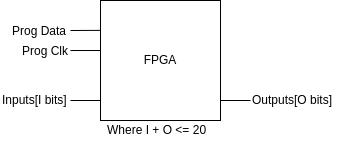
\includegraphics[width=0.5\textwidth]{toplevel}
    \caption{Top level block diagram}
    \label{fig:toplevel}
\end{figure}

\begin{figure}[h]
    \centering
    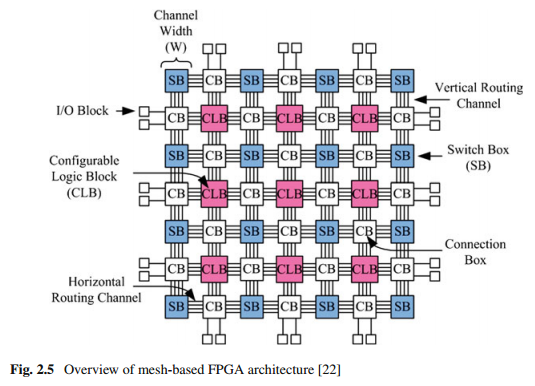
\includegraphics[width=0.5\textwidth]{generalarch}
    \caption{General island-style FPGA architecture}
    \label{fig:generalarch}
\end{figure}

\begin{figure}[h]
    \centering
    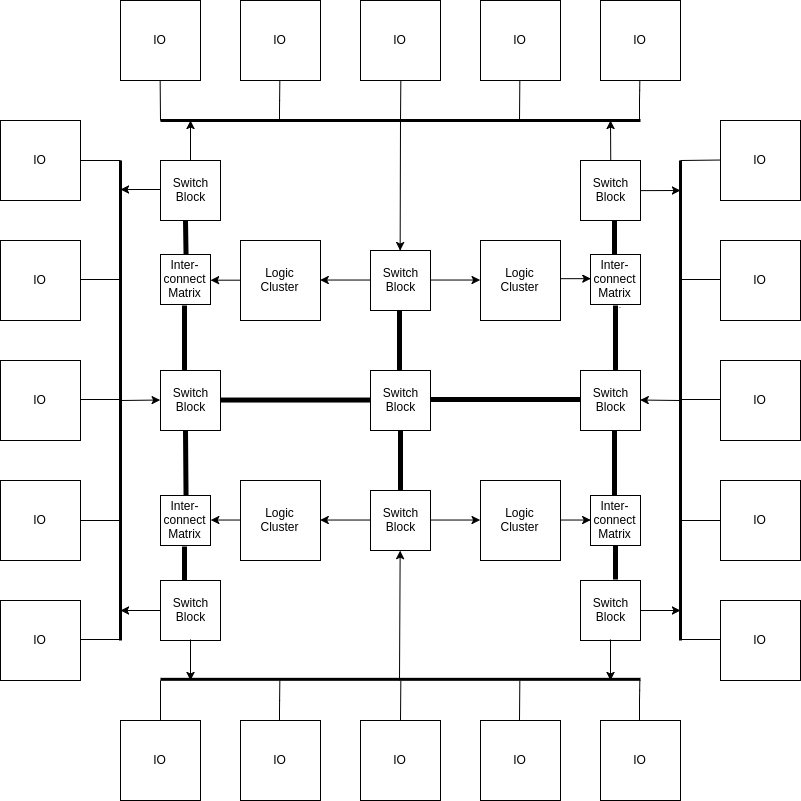
\includegraphics[width=0.75\textwidth]{arch}
    \caption{High level block diagram (no programming signals)}
    \label{fig:arch}
\end{figure}

\begin{figure}[h]
    \centering
    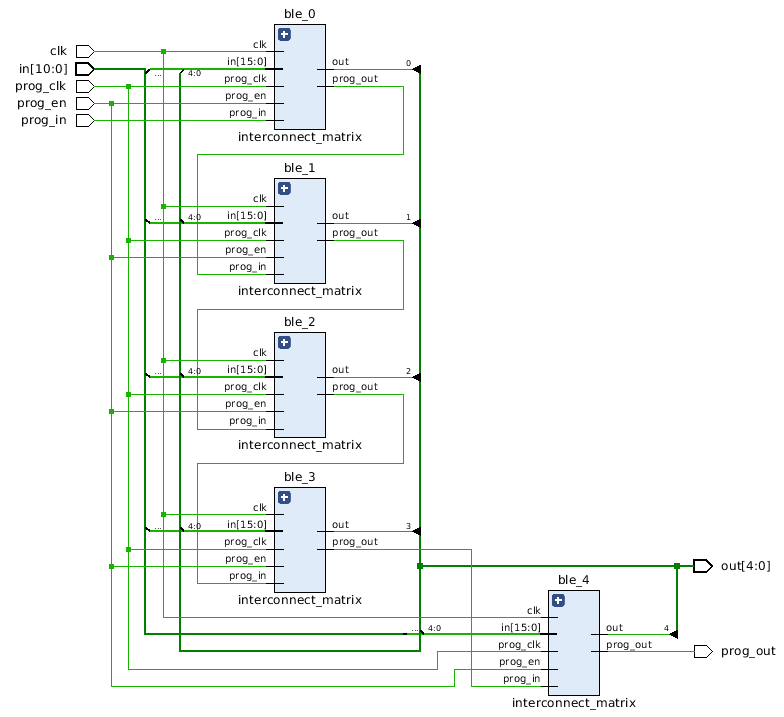
\includegraphics[width=0.5\textwidth]{circuit_toplevel}
    \caption{Logic cluster circuit diagram}
    \label{fig:circuit_toplevel}
\end{figure}

The design of the BLE block is very basic. The block design can be seen in Figure 
2.7 and the verilog code can be found in Figure 2.8. The BLE contains 3 2-bit muxes
, 1 16-bit mux, and 2 19 bit shift registers, 16 bits of which are used in the 4-
LUT. The remaining 3 bits are used to: enable the feedback path from the flip flop 
to input A of the 4-LUT, enable the use of input D as the enable input to the flip 
flop, and lastly to select the flip flop as output or the 4-LUT as the output. This 
design will aid in simplicity of circuit verification and in implementation routing
. The addition of two sets of shift registers was discovered to be required during 
simulation as the circuit would enter into invalid states while being programmed. 
To combat this problem, there are two banks of shift registers. The first is used 
only while the device is being programed (as told by the prog{\_}enable signal). The 
second is only filled when the final control signals are in the programming shift 
registers (falling edge of prog{\_}enable signal).

\begin{figure}[h]
    \centering
    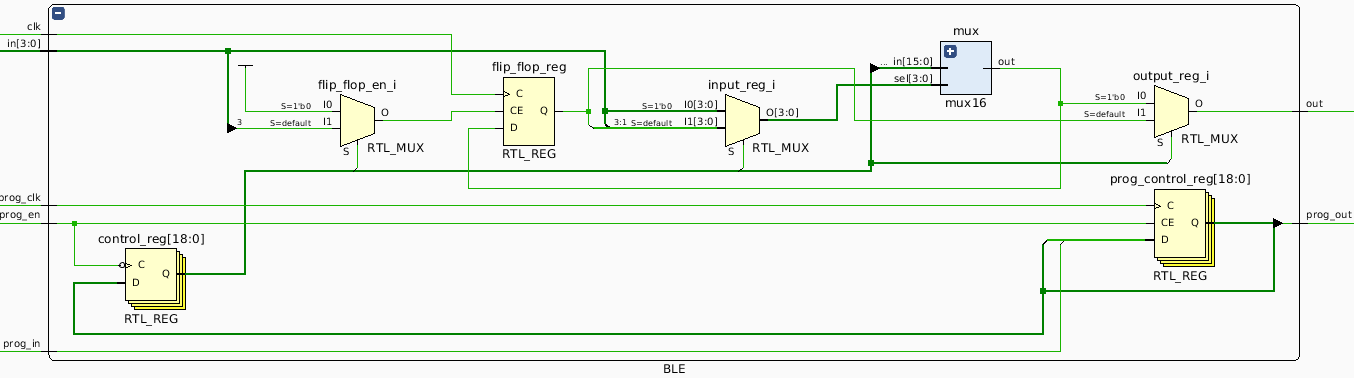
\includegraphics[width=\textwidth]{circuit_ble}
    \caption{Basic logic element circuit diagram}
    \label{fig:ble}
\end{figure}

\begin{figure}[h]
    \lstinputlisting[language=Verilog]{../src/logic_element.v}
    \caption{Basic logic element code}
    \label{code:ble}
\end{figure}

The interconnect matrix was also approached with a very basic implementation in mind
. A large design decision was made to describe the interconnect matrix in verilog 
instead of utilizing a mixed flow transistor level design. This allowed an extremely 
simple design of having four 16-bit muxes tied to each BLE. In addition to being 
simple to design, the choice of verilog also made the use of a HDL static analysis 
tool possible which made verification a much simpler task. Each mux is programed 
to pass a single signal for the entire programmed operation of the device. This leads 
to a programming bit count of 80 (5 BLEs * 4 Inputs per BLE * 4 programming bits 
per 16-bit mux). It is yet to be seen how this design performs in comparison to a 
transistor level design.


\section{Circuit Validation}

\section{Tools}

\section{Conclusion}
\end{document}
              
            
